\documentclass[11pt]{article}

% ── Layout & typography ─────────────────────────────────────────────────
\usepackage[margin=2.2cm]{geometry}
\usepackage[T1]{fontenc}
\usepackage[utf8]{inputenc}
\usepackage{lmodern}
\usepackage{microtype}
\usepackage{setspace}\setstretch{1.15}
\usepackage{parskip}
\usepackage{lineno}\linenumbers
\usepackage[font=small,labelfont=bf]{caption}
\setlength{\emergencystretch}{2em}

% ── Math, figures, references ──────────────────────────────────────────
\usepackage{amsmath}
\usepackage{amssymb}
\usepackage{graphicx}
\usepackage{comment}
\usepackage{url}
\usepackage{xcolor}
\usepackage[colorlinks=true, allcolors=blue!50!black, citecolor=teal!60!black]{hyperref}
\usepackage{xr-hyper}                             % cross-document refs (e.g. main text labels)
\externaldocument{main}                            % reads main.aux if present
\usepackage[
    backend=biber,
    style=authoryear,
    sorting=nyt,
    natbib=true
]{biblatex}
\addbibresource{biblio.bib}

\graphicspath{{./}{figures/}{SI_figures/}{img/}}

% Supplementary figures numbered S1, S2, ... (also picked up by xr-hyper in main.tex)
\renewcommand{\thefigure}{S\arabic{figure}}


\title{Supplementary Information \\
Convective Organization \\ as Markov Trajectories in Latent Space}
\author{Sophie Abramian, Olivier Pauluis, Pierre Gentine}
\date{June 2026}

\begin{document}

\maketitle


\tableofcontents

\newpage

\section{Training and Validation Losses}


The model is trained for 500 epochs by minimizing a composite objective that combines data fidelity, latent-space regularization, structural contrast, and discrete dynamical consistency. The total loss is given by
\[
\mathcal{L} =
\|X - \hat{X}\|^2
+
\frac{1}{2}\sum_{i=1}^d
\left(
\mu_i^2 + \sigma_i^2 - \log \sigma_i^2 - 1
\right)
-
\mathcal{L}_{\mathrm{Dice}}
-
\sum_{i,j}
s_t(i)\, s_{t+1}(j)\, \log T_{ij},
\]
where the first term corresponds to the reconstruction error, the second term is the Kullback--Leibler divergence enforcing regularization of the continuous latent variables, the third term is a Dice-based contrastive regularization promoting structural separation between latent states, and the final term enforces temporal consistency through a Markov state-transition likelihood.

Figure~\ref{fig:loss_curves} shows the evolution of the total loss and its individual components for both training and validation data. To improve readability, the loss decomposition is shown separately for training and validation. All loss components are displayed on a logarithmic scale to highlight their relative contributions and convergence behavior over the course of training.

The close agreement between training and validation curves across all loss terms indicates stable multi-objective optimization and good generalization, with no evidence of late-epoch overfitting in either the continuous or discrete components of the model.


\begin{figure}
    \centering
    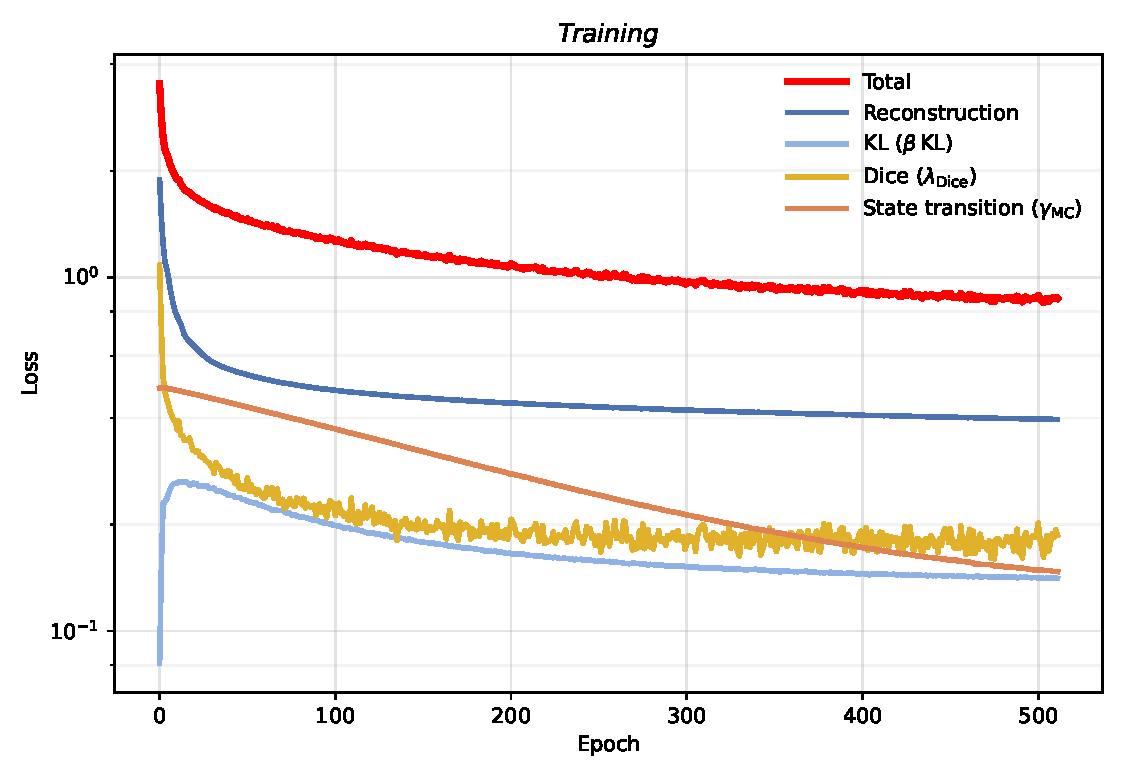
\includegraphics[width=0.49\textwidth]{training_loss.pdf}
    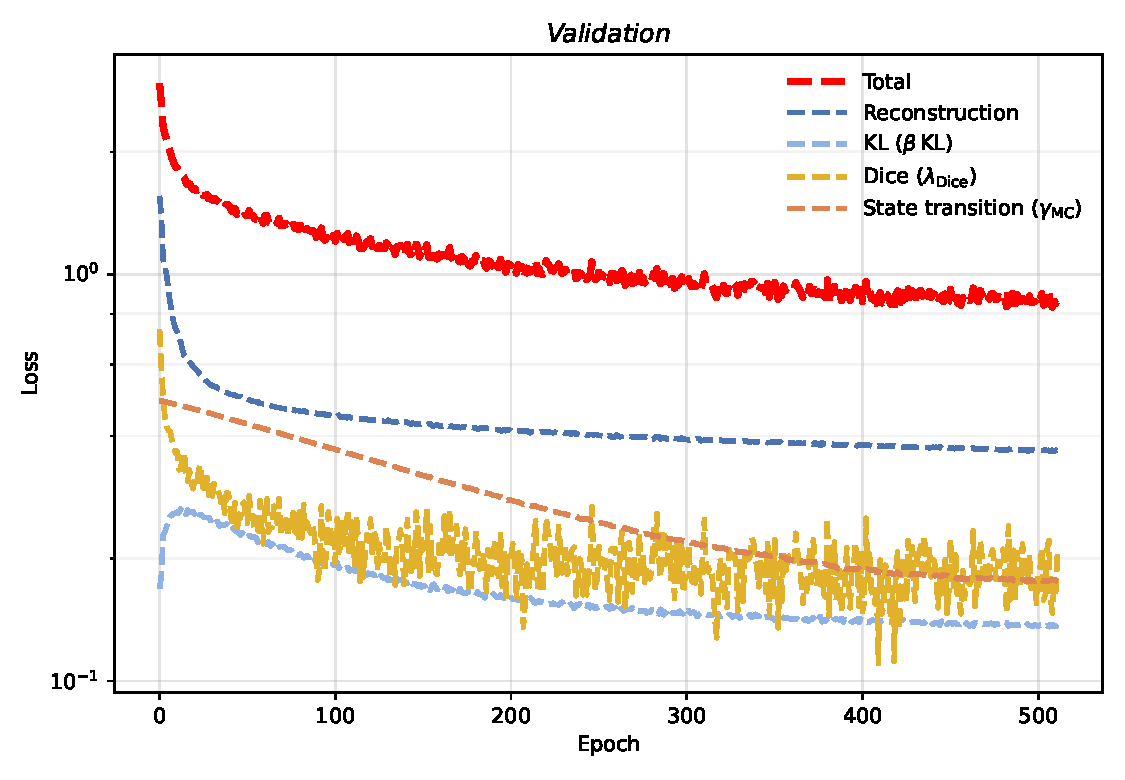
\includegraphics[width=0.49\textwidth]{validation_loss.pdf}
    \caption{Training and validation loss decomposition for the proposed hybrid VAE--Markov model.
Loss components are shown on a logarithmic scale to emphasize their relative magnitudes and convergence behavior across epochs. The consistency between training and validation curves suggests stable optimization and robust generalization across reconstruction, latent regularization, structural contrast, and state-transition dynamics.}
    \label{fig:loss_curves}
\end{figure}



\section{Reconstruction Skills}

To assess the reconstruction capabilities of the model, we show representative examples of reconstructed isentropic mass flux diagrams alongside their corresponding ground-truth fields. Examples are randomly selected from the dataset, with snapshots drawn from different latent states in order to provide an overview of reconstruction performance across the full range of learned dynamical regimes.

For each selected state, a single latent embedding is sampled at random and decoded to produce a reconstructed mass flux field. The reconstructed fields are then compared to the original input fields at the same time index. All examples are displayed using identical color scales to allow direct visual comparison of spatial structure, amplitude, and sign.

As illustrated in Figure~\ref{fig:reconstruction}, the model is able to faithfully recover the dominant spatial patterns and vertical–isentropic structure of the mass flux anomalies across states, while preserving large-scale coherence and sharp gradients. Notably, the reconstructed fields often appear smoother than the corresponding ground-truth inputs, with reduced small-scale variability. This behavior is consistent with the probabilistic nature of variational autoencoders, which tend to suppress high-frequency noise while retaining the most informative components of the signal. Such denoising is indicative of a meaningful and structured latent representation rather than simple memorization of the input fields.

\begin{figure}
    \centering
    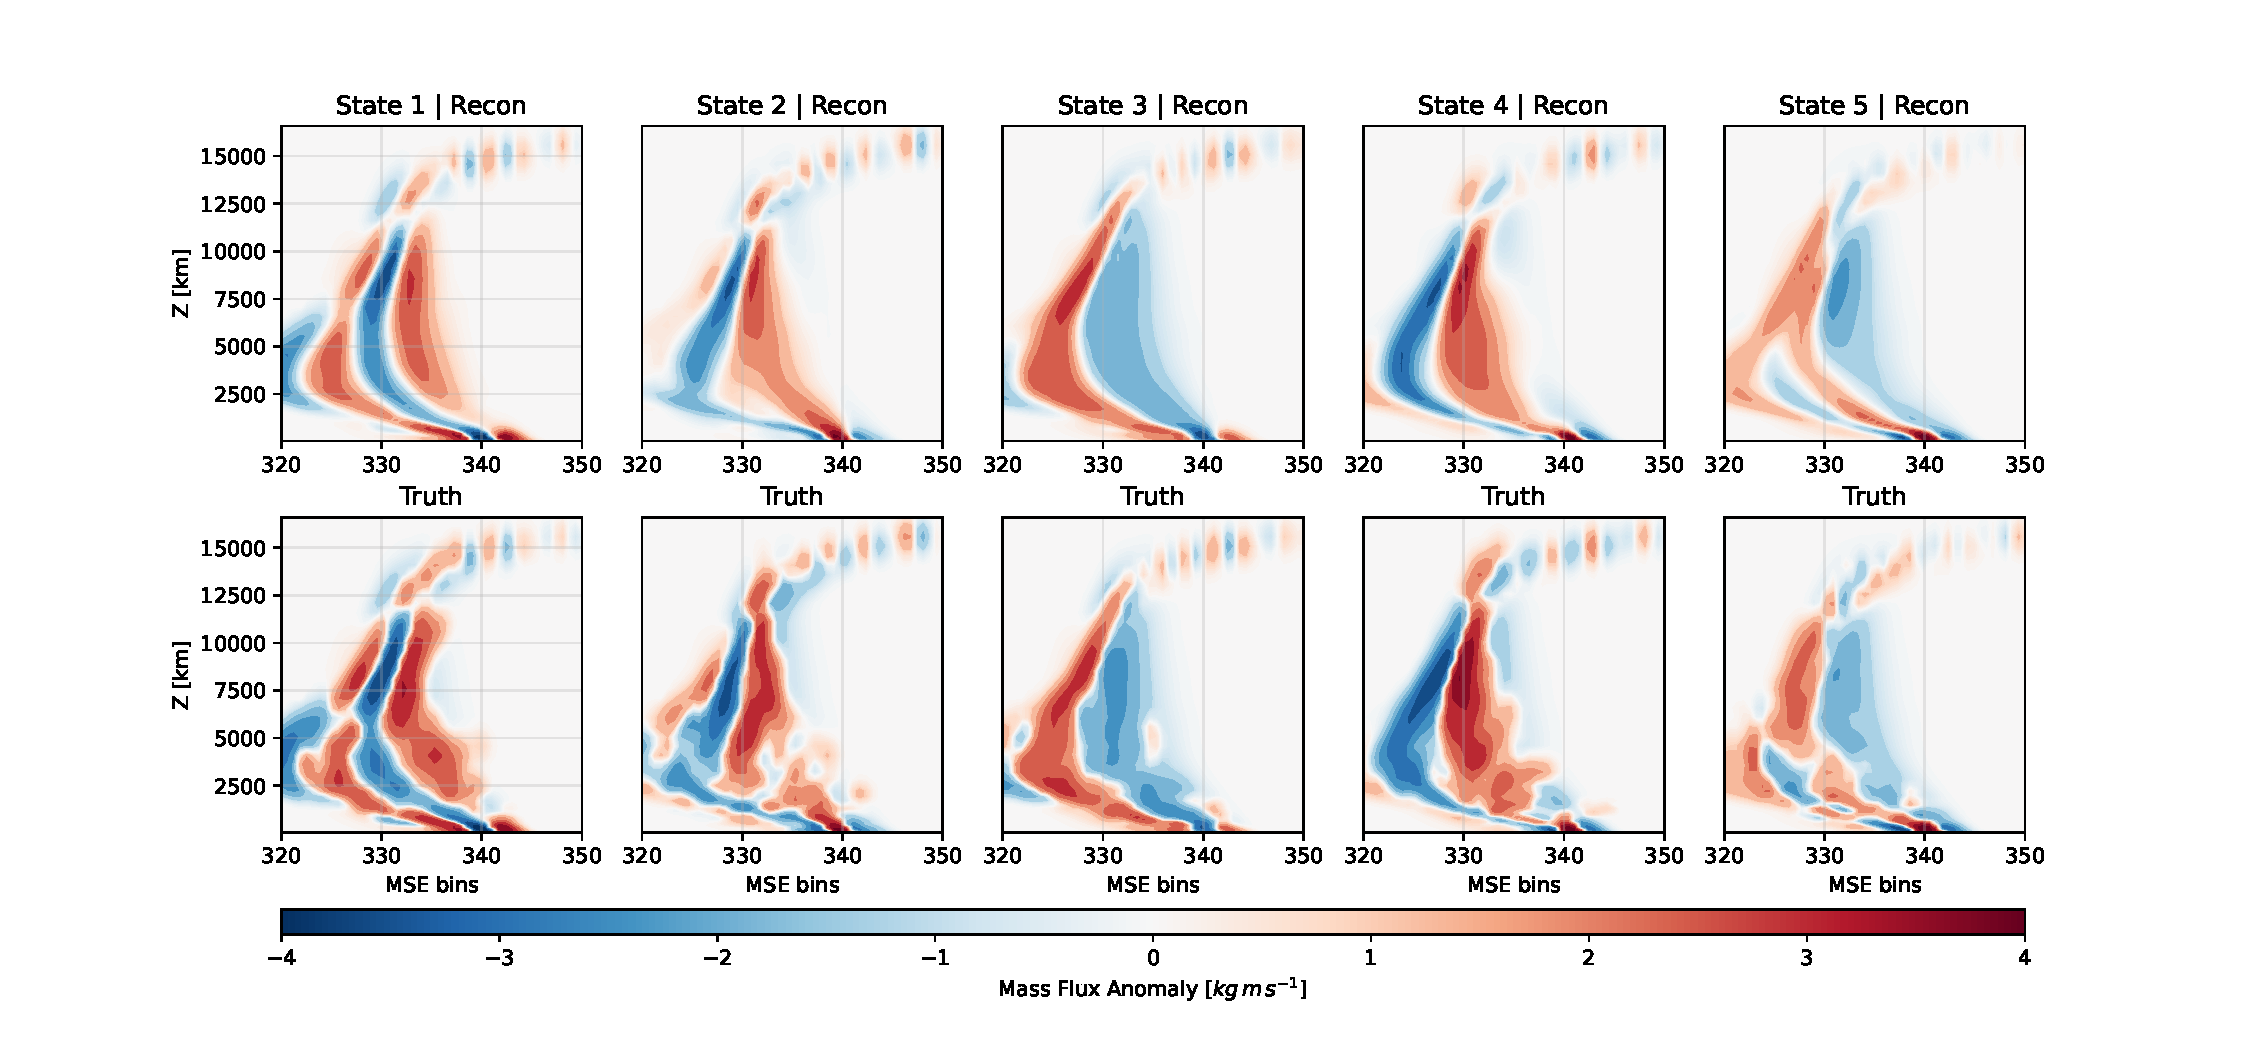
\includegraphics[width=\textwidth]{reconstruction.pdf}
    \caption{Examples of reconstructed and true isentropic mass flux diagrams for randomly selected snapshots from different latent states.
Each column corresponds to a distinct latent state, with one randomly chosen time index per state. The top row shows reconstructions obtained by decoding the latent embedding, while the bottom row shows the corresponding ground-truth fields. All panels use the same color scale, highlighting the model's ability to recover the dominant spatial structure, amplitude, and vertical organization of mass flux anomalies across a range of dynamical regimes.}
    \label{fig:reconstruction}
\end{figure}





\section{Sensitivity test to hyperparameters}
\subsection*{Latent dimension}

We compare the evolution of the reconstruction loss during training for models with different latent dimensionalities equal to 4, 8 (the one chosen) and 16 (Fig.~\ref{fig:latent_dim_sensitivity}). Increasing the latent dimension systematically reduces the reconstruction error and accelerates convergence, reflecting the increased expressive capacity of the latent space. However, beyond a moderate latent size, improvements become marginal, suggesting diminishing returns in reconstruction quality. This supports the choice of an intermediate latent dimension equal to 8 as a trade-off between representational power and model complexity. The logarithmic scale highlights early-epoch differences and stabilisation behaviour across configurations.

\begin{figure}
    \centering
    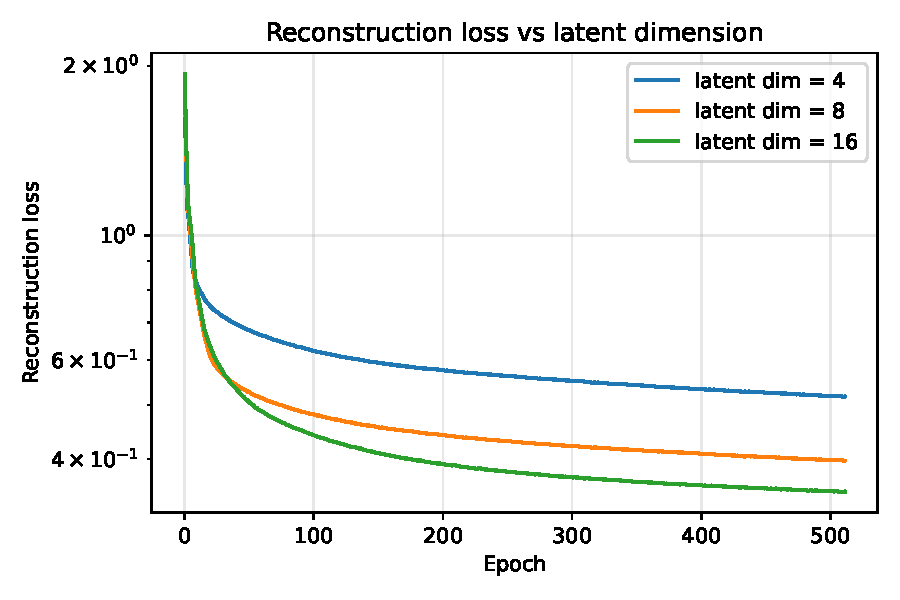
\includegraphics[width=0.7\textwidth]{latent_dim_sensitivity.pdf}
    \caption{Curves show the reconstruction loss as a function of epoch for models with varying latent space sizes. The loss is displayed on a logarithmic scale.}
    \label{fig:latent_dim_sensitivity}
\end{figure}



\subsection*{Number of clusters}

We assess the sensitivity of the latent-space organisation to the prescribed number of discrete clusters by training models with 3, 7, and 10 latent states alongside the 5-state model used in the main text (Fig.~\ref{fig:cluster_sensitivity}). Across all configurations, the separation between organised and unorganised trajectories remains robust, indicating that the inferred dynamical pathways are not an artefact of a particular cluster partitioning. The split is already clearly captured at three clusters: a single organised cluster, a single unorganised cluster, and an intermediate suppressed-convection cluster recover the dominant route through state space. Increasing $K$ to seven or ten refines these regimes into sub-types (multiple sub-organised, dry, or stratiform-leaning sub-clusters) but does not introduce new dynamical regimes; the additional states appear primarily as further subdivisions inside the same two basins. We retain $K=5$ as the working partition because it resolves the two organised regimes (organised-deep Cluster~1 and stratiform-like Cluster~2) and the two unorganised regimes (active-unorganised Cluster~4 and shallow-congestus Cluster~5) without proliferating dynamically redundant sub-states, and because all four headline findings of the main text---the intensity/organisation axis structure, the existence of an organised cluster, the two-regime split carried by the second eigenmode, and the residual non-Markovianity of the organised cluster---survive unchanged across the comparator set.

\begin{figure}
    \centering
    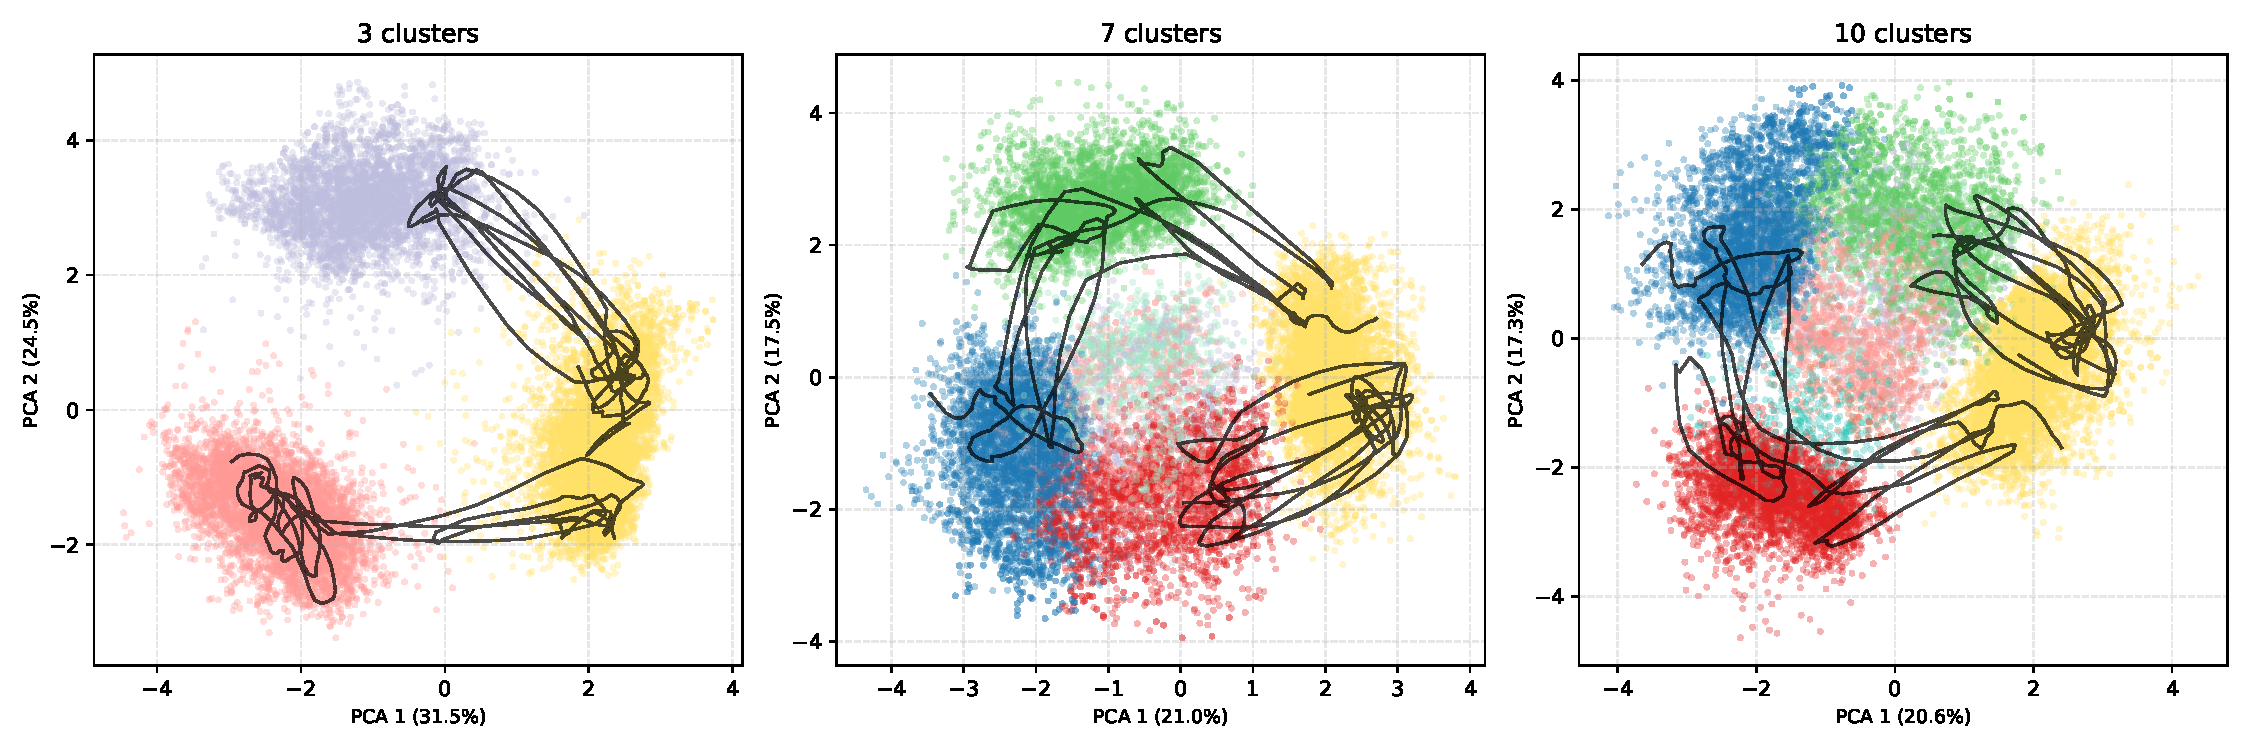
\includegraphics[width=\textwidth]{cluster_sensitivity.pdf}
    \caption{Principal component projections of the latent embeddings for different numbers of discrete latent states.
Panels show the first two principal components of the latent representations for models trained with 3, 7, and 10 clusters (left to right), using a fixed latent dimension of 8. Points are coloured by inferred latent state. Solid black curves indicate smoothed latent-space trajectories from the two representative intervals (strongly organised and weakly organised) used in the main text, allowing the same trajectories to be inspected against each alternative partition.}
    \label{fig:cluster_sensitivity}
\end{figure}

\subsection*{Three-dimensional PCA projection}

The 2D PCA projection in the main text (Fig.~\ref{fig:clusters}) suggests partial overlap between some clusters. Expanding to three components shows that clusters which appear to overlap in 2D are separated along higher-order axes (Fig.~\ref{fig:pca_3d}).

\begin{figure}
    \centering
    \IfFileExists{figures/pca_3d.pdf}{%
        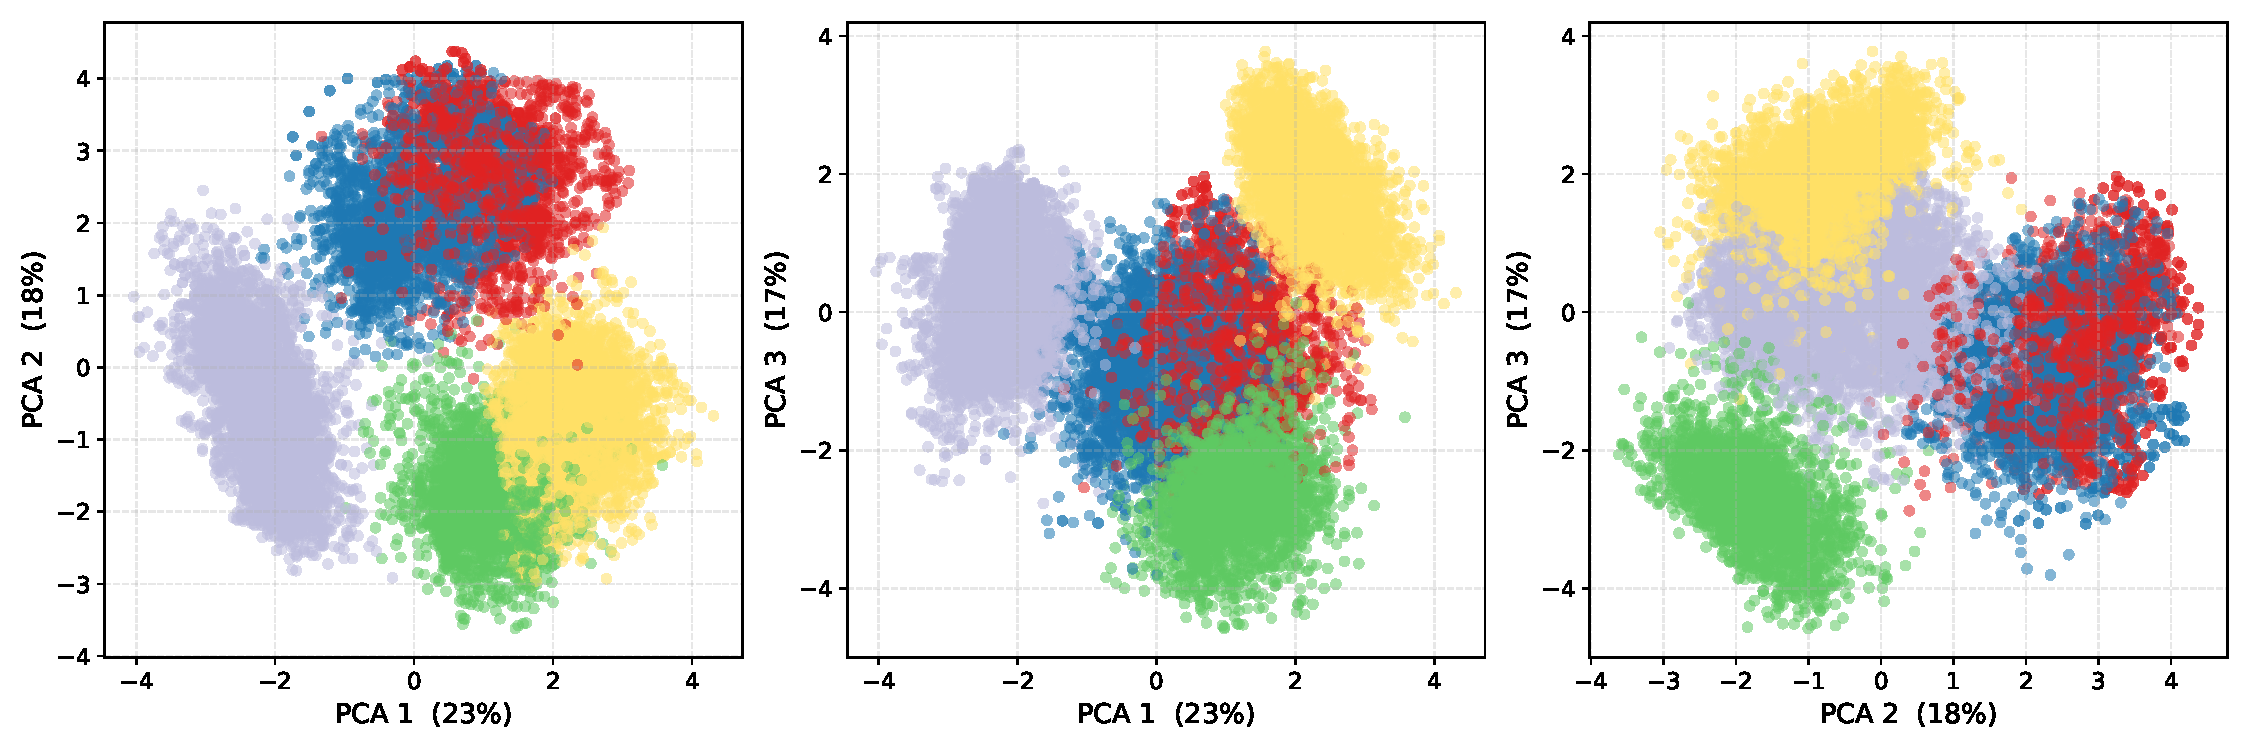
\includegraphics[width=\textwidth]{pca_3d.pdf}%
    }{%
        \framebox[0.6\textwidth]{\parbox[c][4cm][c]{0.55\textwidth}{\centering\itshape
        Figure missing: regenerate \texttt{pca\_3d.pdf} by running \texttt{figures\_si.ipynb}.}}%
    }
    \caption{\textbf{Three-dimensional PCA projection of the latent space.} All three pairwise projections (PCA~1 vs.~PCA~2, PCA~1 vs.~PCA~3, PCA~2 vs.~PCA~3) of the leading three principal components, coloured by latent state. Clusters that appear to overlap in the 2D projection used in the main text are separated along higher-order components.}
    \label{fig:pca_3d}
\end{figure}


\section{Contrastive regularization of state assignments}

To regularize the latent state assignment and prevent state collapse, we introduce a contrastive loss that enforces consistency between discrete state probabilities and the structural similarity of the underlying mass-flux anomaly fields.

\paragraph{Structural similarity.}
Given a sample $i$ with reconstructed mass-flux anomaly field $x_i(\mathbf{r})$, we define a discrete structural representation by thresholding the field into three classes using fixed values $\{-1.5,\,1.5\}$:
\[
m_i(\mathbf{r}) =
\begin{cases}
0, & x_i(\mathbf{r}) < -1.5, \\
1, & -1.5 \le x_i(\mathbf{r}) \le 1.5, \\
2, & x_i(\mathbf{r}) > 1.5.
\end{cases}
\]
For each class $c \in \{0,1,2\}$, we define the corresponding binary mask
\[
M_i^c(\mathbf{r}) = \mathbf{1}\!\left[m_i(\mathbf{r}) = c\right].
\]

The structural similarity between two samples $i$ and $j$ is quantified using a macro-averaged Dice coefficient,
\[
\mathrm{Dice}(i,j)
=
\frac{1}{3}
\sum_{c=0}^{2}
\frac{2\,|M_i^c \cap M_j^c|}{|M_i^c| + |M_j^c|},
\]
with the convention that the Dice score for class $c$ is set to $1$ when both masks are empty. We define the corresponding Dice distance as
\[
d_{ij} = 1 - \mathrm{Dice}(i,j),
\]
so that $d_{ij} \in [0,1]$, with small values indicating high structural similarity.

\paragraph{Probabilistic state agreement.}
Let $s_i \in \mathbb{R}^K$ denote the soft state assignment for sample $i$, where $s_i(k)$ is the probability of occupying state $k$. The probability that two samples share the same state is defined as
\[
p_{\mathrm{same}}(i,j) = \sum_{k=1}^K s_i(k)\, s_j(k),
\qquad
p_{\mathrm{diff}}(i,j) = 1 - p_{\mathrm{same}}(i,j).
\]

\paragraph{Soft contrastive windows.}
We distinguish three regimes based on the Dice distance $d_{ij}$: a cohesion regime for structurally similar pairs, a separation regime for dissimilar pairs, and an intermediate regime. These regimes are implemented using linear soft windows with thresholds $\tau_{\mathrm{coh}}$ and $\tau_{\mathrm{sep}}$ and width parameter $w$:
\[
w_{\mathrm{coh}}(d_{ij}) =
\mathrm{clip}\!\left(\frac{\tau_{\mathrm{coh}} - d_{ij}}{w},\,0,\,1\right),
\]
\[
w_{\mathrm{sep}}(d_{ij}) =
\mathrm{clip}\!\left(\frac{d_{ij} - \tau_{\mathrm{sep}}}{w},\,0,\,1\right),
\]
\[
w_{\mathrm{mid}}(d_{ij}) =
\mathrm{clip}\!\left(\frac{d_{ij} - \tau_{\mathrm{coh}}}{w},\,0,\,1\right)
\cdot
\mathrm{clip}\!\left(\frac{\tau_{\mathrm{sep}} - d_{ij}}{w},\,0,\,1\right).
\]

\paragraph{Pairwise penalties.}
For each sampled pair $(i,j)$, we define three complementary penalties:
\begin{itemize}
\item \textbf{Cohesion penalty} (similar structures assigned to different states):
\[
\mathcal{L}_{\mathrm{coh}}(i,j)
=
w_{\mathrm{coh}}(d_{ij}) \, \bigl(1 - p_{\mathrm{same}}(i,j)\bigr),
\]
\item \textbf{Separation penalty} (dissimilar structures assigned to the same state):
\[
\mathcal{L}_{\mathrm{sep}}(i,j)
=
w_{\mathrm{sep}}(d_{ij}) \, p_{\mathrm{same}}(i,j),
\]
\item \textbf{Mid-range uncertainty penalty} (ambiguous similarity with uncertain assignment):
\[
\mathcal{L}_{\mathrm{mid}}(i,j)
=
\lambda_{\mathrm{mid}}\,
w_{\mathrm{mid}}(d_{ij})\,
p_{\mathrm{same}}(i,j)\, p_{\mathrm{diff}}(i,j),
\]
where $\lambda_{\mathrm{mid}}$ controls the strength of the uncertainty penalty.
\end{itemize}

\paragraph{Final contrastive loss.}
The total Dice-based contrastive loss is obtained by averaging over a set $\mathcal{P}$ of randomly sampled pairs within each batch:
\[
\mathcal{L}_{\mathrm{Dice}}
=
\frac{1}{|\mathcal{P}|}
\sum_{(i,j)\in\mathcal{P}}
\Bigl(
\mathcal{L}_{\mathrm{coh}}(i,j)
+
\mathcal{L}_{\mathrm{sep}}(i,j)
+
\mathcal{L}_{\mathrm{mid}}(i,j)
\Bigr).
\]

This loss enforces that latent states correspond to consistent spatial structures of positive and negative mass-flux anomalies, while avoiding degenerate solutions in which all samples collapse onto a single state. Importantly, the loss operates purely on structural information and does not constrain anomaly amplitude or fine-scale intensity.


\section{Markov Chain and the Koopman operator}

The Markov transition model introduced above naturally emerges from the framework of Koopman operator theory, which provides a linear, generally infinite-dimensional, representation of nonlinear dynamical systems by acting on observables---functions of the system state---rather than on the state variables themselves.

Let $x_t \in \mathcal{X}$ denote the full convective state of the system at time $t$. We approximate the Koopman observable with a universal function approximator: a VAE-based neural network, which maps each convective snapshot to a latent representation $z_t = E(x_t)$ and subsequently to a probability vector
\[
\pi(x_t) = (\pi_1(x_t), \ldots, \pi_K(x_t)) \in \Delta^{K-1},
\]
where $\pi_i(x_t) = \mathbb{P}(s_t = i \mid x_t)$ denotes the probability of assignment to convective state $i$. The components of $\pi$ thus define a finite set of learned, smooth observables $f_i = \pi_i \circ E$, parameterized by the VAE encoder $E$.

Under the assumption that the evolution of these observables is approximately Markovian, the Koopman operator $\mathcal{K}$ acts on an observable $f$ according to
\[
(\mathcal{K} f)(x_t) = \mathbb{E}\!\left[ f(x_{t+1}) \mid x_t \right].
\]
Restricting $\mathcal{K}$ to the finite-dimensional subspace spanned by $\{ f_i \}_{i=1}^K$, its action is approximated by a stochastic transition matrix $T$, such that
\[
\mathbb{E}\!\left[ \pi(x_{t+1}) \mid \pi(x_t) \right] \;\approx\; T \, \pi(x_t),
\]
where $T$ represents the action of the stochastic Koopman operator projected onto the subspace defined by the VAE-learned observables.

The spectral properties of $T$ provide insight into the intrinsic dynamics of the reduced system. The leading eigenvalue $\lambda_1 = 1$ corresponds to the stationary distribution over convective states, while subdominant eigenvalues characterize slowly decaying modes associated with regime persistence and long-lived correlations. Complex-conjugate eigenvalue pairs indicate oscillatory behavior or preferred cyclic transition pathways in the reduced state space.

This formulation establishes a principled connection between the VAE-based universal approximation of Koopman observables and data-driven stochastic modeling of convective variability, enabling the identification of dominant regimes, transition pathways, and intrinsic time scales of convective organization.

Time series of individual realizations confirm that system trajectories cluster along the two dominant pathways identified from the leading eigenmode of $T$ (Fig.~\ref{fig:trajectories}); these are the same trajectories overlaid on the latent space in the main text.

\begin{figure}
    \centering
    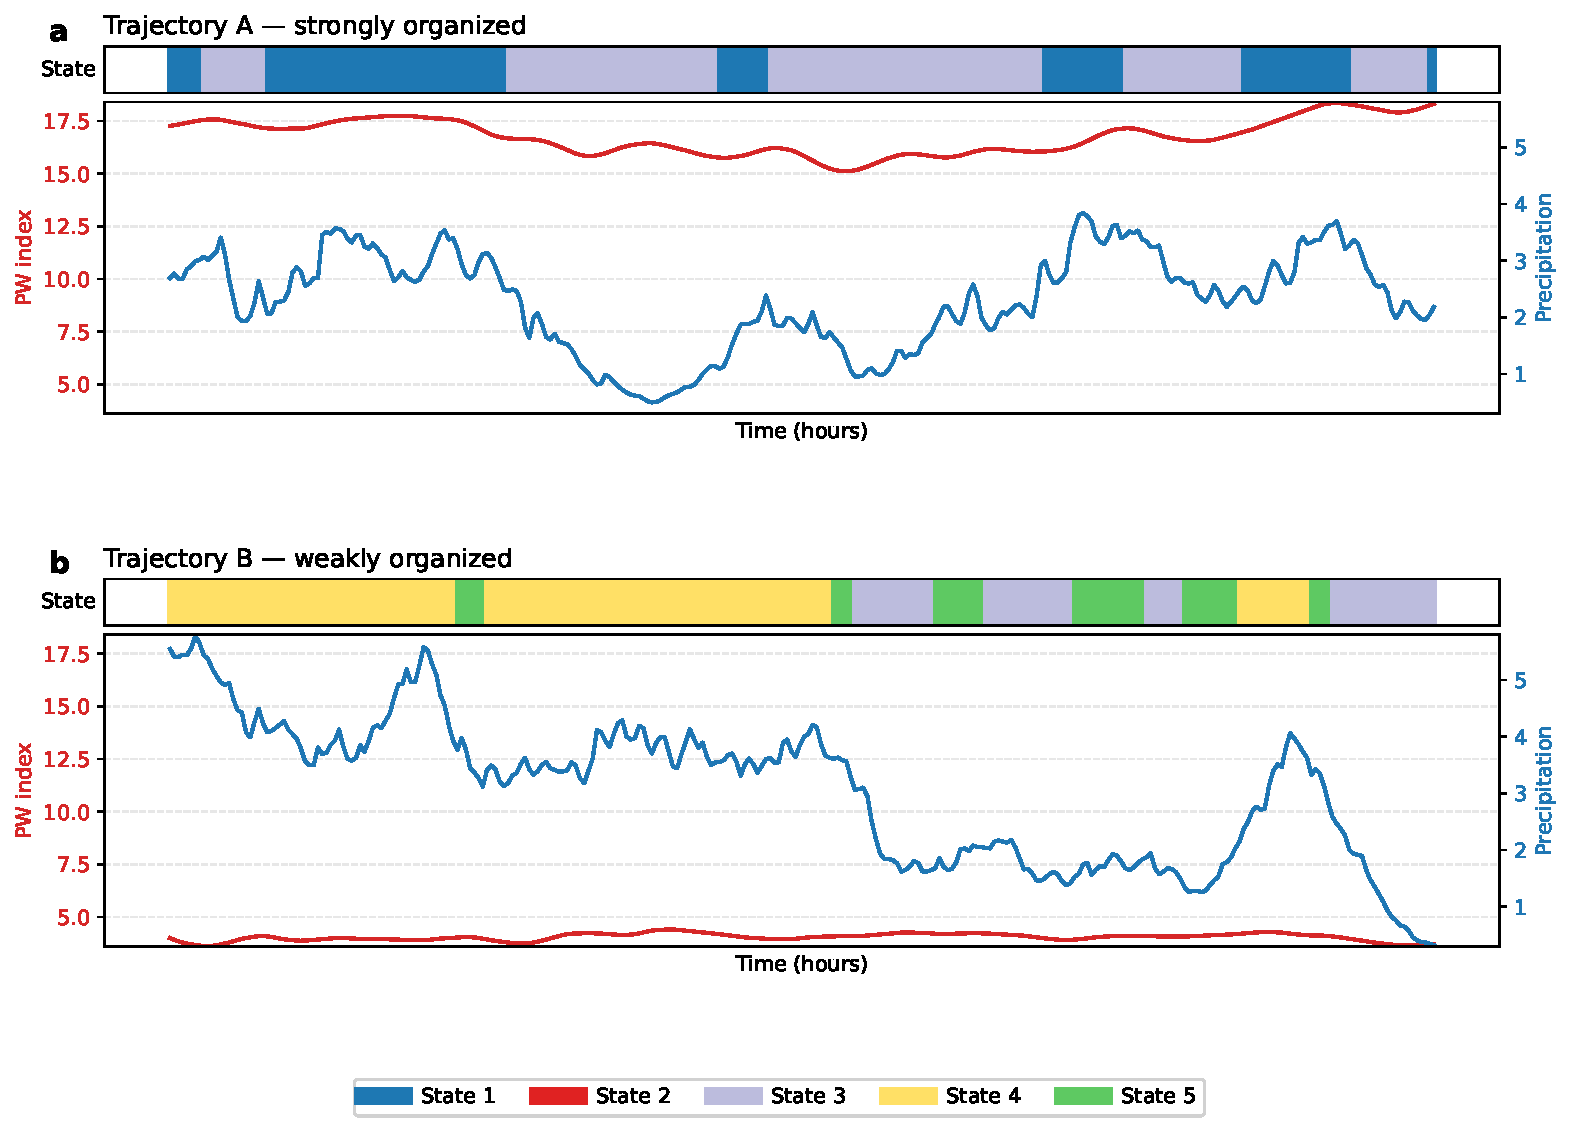
\includegraphics[width=\textwidth]{fig8_trajectories.pdf}
    \caption{\textbf{Example trajectories.} Domain-wide precipitable water (blue, left axis) and precipitation (red, right axis) over two 10-hour intervals, with the latent state at each time step indicated by the colored stripe above each panel. \textbf{(a)} Strongly-organized pathway. \textbf{(b)} Weakly-organized pathway.}
    \label{fig:trajectories}
\end{figure}

\section{Canonical representations of latent states}

In order to define a canonical physical representation for each latent state, we construct state-conditional mean fields using the most representative samples associated with that state. Specifically, for each state, we identify a subset of samples closest to the state barycenter in the reduced PCA–latent space and use these samples as representative realizations of the corresponding dynamical regime.

For the isentropic mass flux, we compute the mean physical field $\langle x \rangle$ by averaging the selected representative samples directly in data space. In parallel, we compute the mean latent embedding $\langle z \rangle$ over the same samples and decode it using the trained decoder, yielding $\mathrm{Dec}(\langle z \rangle)$. These two constructions correspond respectively to averaging in physical space and averaging in latent space.

Figure~\ref{fig:state_means} shows that $\langle x \rangle$ and $\mathrm{Dec}(\langle z \rangle)$ provide consistent canonical representations of each latent state. Their close agreement indicates that the latent space organizes samples in a physically meaningful manner, such that state-specific structures are preserved under both averaging procedures. As expected for a variational autoencoder, the decoded representations exhibit a mild smoothing relative to the direct physical averages, while retaining the dominant vertical and isentropic patterns characteristic of each state.

To further illustrate the physical coherence of the latent states, we also show multi-variable canonical composites constructed by averaging additional atmospheric fields over the same representative samples for each state (Fig.~\ref{fig:state_multivar}).


\begin{figure}
    \centering
    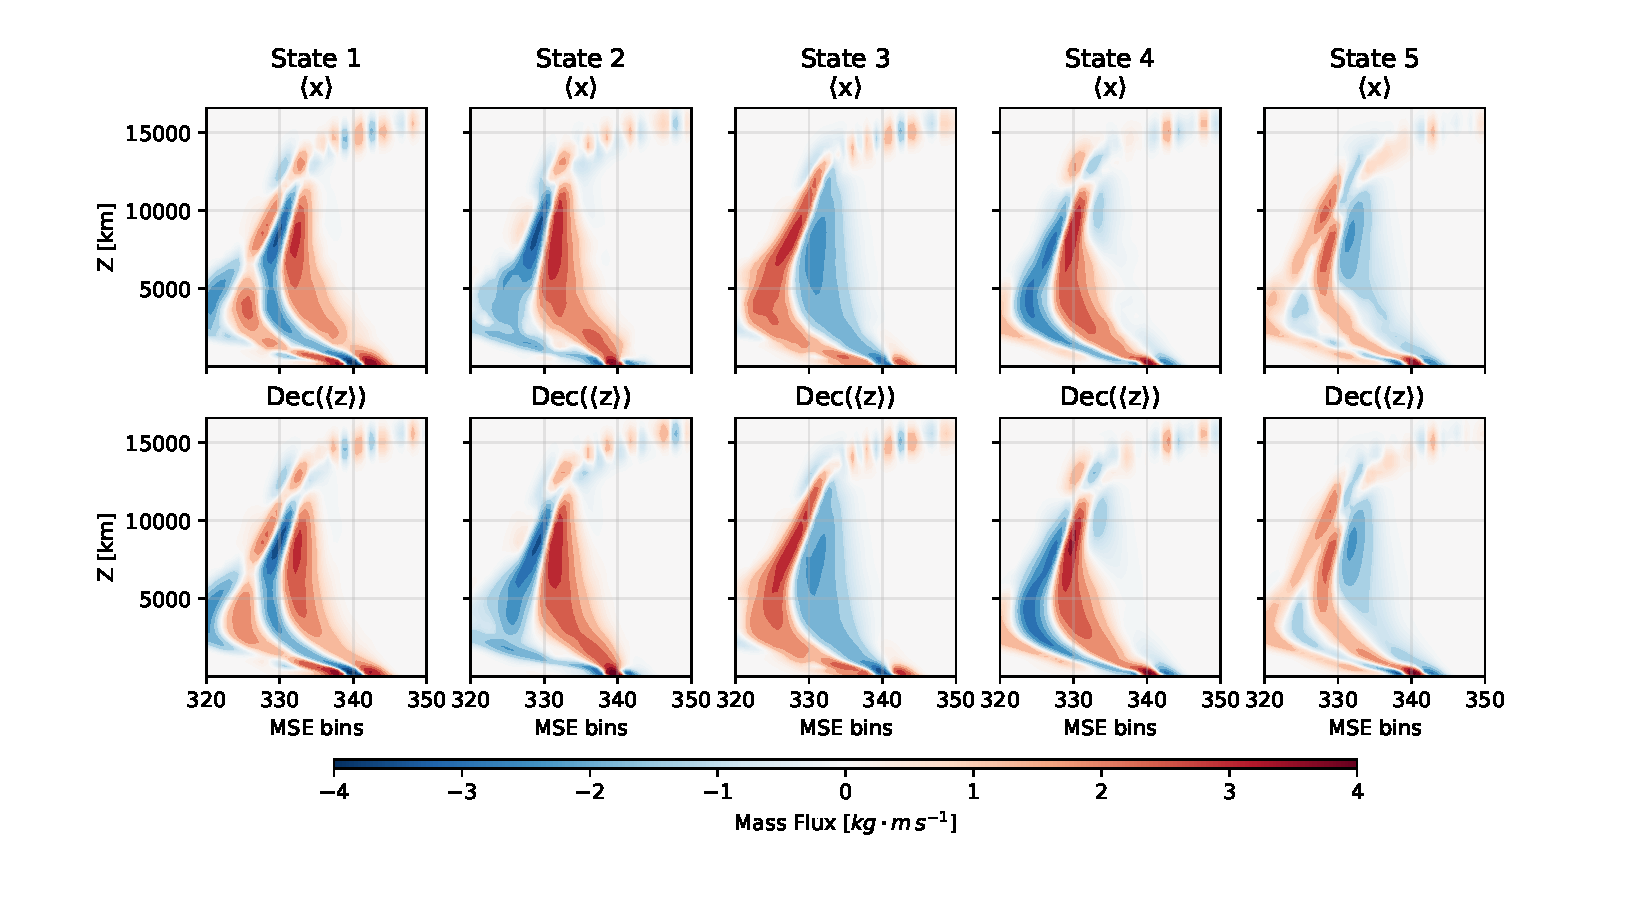
\includegraphics[width=\textwidth]{canonical_representative.pdf}
    \caption{Canonical isentropic mass flux representations for each latent state.
    Each column corresponds to a latent state, using the most representative samples closest to the state barycenter in latent space. The top row shows the mean mass flux field obtained by averaging these samples directly in physical space ($\langle x \rangle$), while the bottom row shows the reconstruction obtained by decoding the mean latent embedding of the same samples ($\mathrm{Dec}(\langle z \rangle)$). The close agreement between the two representations demonstrates that averaging in physical space and averaging in latent space yield consistent canonical state patterns, with the reconstructed fields exhibiting the characteristic smoothing expected from a variational autoencoder.}
    \label{fig:state_means}
\end{figure}


\begin{figure}
    \centering
    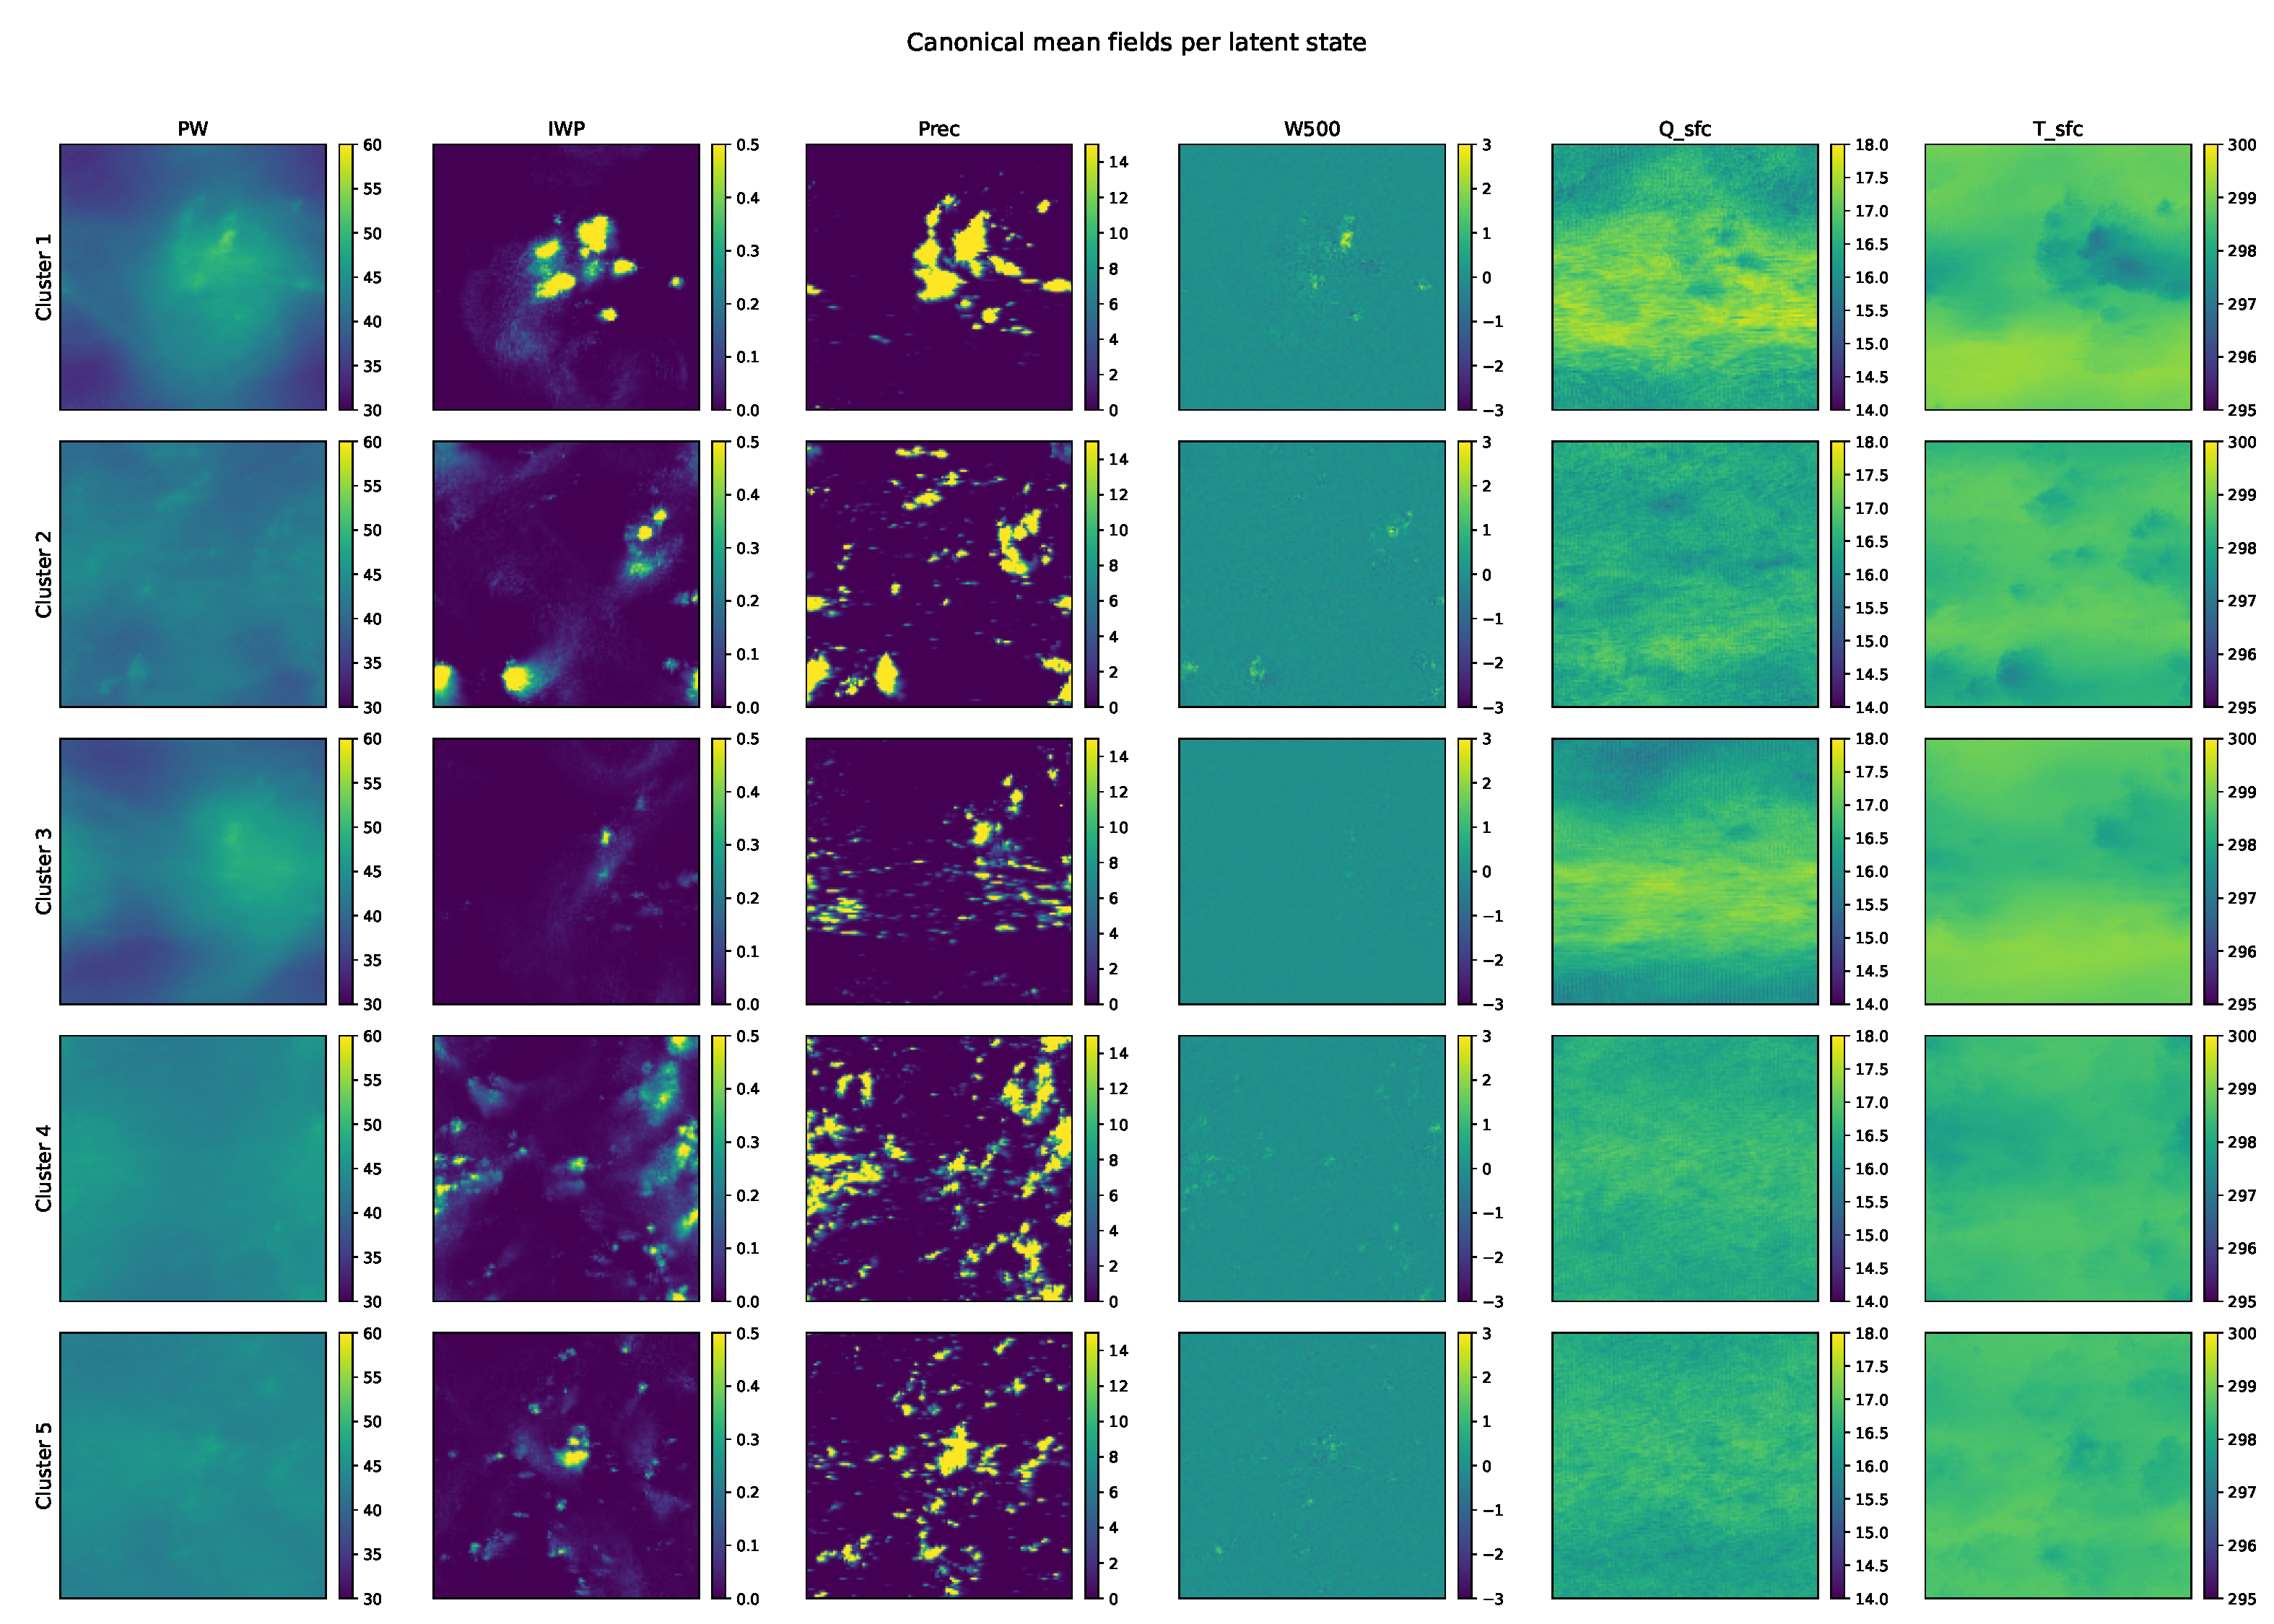
\includegraphics[width=\textwidth]{fields_clusters.pdf}
    \caption{Canonical composite fields for multiple atmospheric variables conditioned on latent states.
    For each latent state (rows), we show mean spatial fields of selected atmospheric variables (columns), computed by averaging the representative samples closest to the state barycenter in latent space. These composites provide a multi-variable physical characterization of each latent state and illustrate that the states correspond to coherent and distinct dynamical regimes.}
    \label{fig:state_multivar}
\end{figure}


\section{Cold pools tracking and activity index}
\subsection*{Cold-pool detection}

Cold pools are detected independently at each model time step from two-dimensional surface temperature field
$T_{abs}(x,y,t)$. The field is first smoothed using a Gaussian filter with standard deviation
$\sigma = 2$--$3$ grid points. Two thresholds are then applied to distinguish cold-pool envelopes and
cores. Grid points satisfying
\begin{equation}
T_{abs}(x,y,t) < \phi_{\mathrm{env}}
\end{equation}
define candidate cold-pool envelopes, while points satisfying
\begin{equation}
T_{abs}(x,y,t) < \phi_{\mathrm{core}}, \qquad \phi_{\mathrm{core}} < \phi_{\mathrm{env}},
\end{equation}
define cold-pool cores.

Envelope grid points are grouped into spatially connected objects using single-linkage agglomerative
clustering with a periodic distance metric to account for domain periodicity. Within each envelope,
core grid points are further clustered using the same approach. Core labels are subsequently propagated
to the surrounding envelope using nearest-neighbor classification, yielding a fully labeled cold-pool
mask at each time step.


\subsection*{Temporal tracking}

Cold-pool objects are tracked forward in time by matching labeled regions between consecutive time
steps based on spatial overlap. For a cold pool with label $i$ at time $t$ and label $j$ at time $t+1$,
the similarity is defined as
\begin{equation}
S_{ij} = \frac{|A_i(t) \cap A_j(t+1)|}{|A_i(t)|},
\end{equation}
where $A_i(t)$ denotes the set of grid points belonging to object $i$ at time $t$. Labels are
propagated when $\max_j S_{ij} > 0.55$, ensuring temporal continuity while allowing for cold-pool
initiation, dissipation, splitting, and merging.

\subsection*{Object-based diagnostics}

Tracked cold pools are characterized using near-surface specific humidity $q_v(x,y,t)$. For each cold
pool $k$ at time $t$, the mean humidity anomaly is defined as
\begin{equation}
\Delta q_v^k(t) = \langle q_v \rangle_k(t) - \langle q_v \rangle_{\mathrm{domain}}(t),
\end{equation}
where angle brackets denote spatial averaging over the cold-pool area and the full domain,
respectively. For each cold pool, we record its lifetime, time-evolving area $A_k(t)$, maximum area,
mean humidity anomaly over its lifetime, and maximum absolute humidity anomaly.

\subsection*{Cold-pool index}

A Cold-Pool Index (CPI) is defined as the total area covered by cold pools at each time step,
\begin{equation}
\mathrm{CPI}(t) = \sum_k A_k(t),
\end{equation}
where the sum is taken over all cold pools present at time $t$. In addition to the raw CPI, normalized,
anomalous, and standardized versions are computed using the temporal mean and standard deviation.


\section{Autocorrelation of state indicators in a Markov chain}

Let $\{X_t\}_{t\ge 0}$ be a discrete-time, stationary Markov chain on a finite
state space $\{1,\dots,K\}$ with transition matrix $\mathbf{T}$ and stationary
distribution $\boldsymbol{\pi}$, satisfying
\begin{equation}
    \mathbf{T}\boldsymbol{\pi} = \boldsymbol{\pi},
    \qquad
    \sum_{i=1}^K \pi_i = 1,
    \qquad
    \pi_i \ge 0.
\end{equation}

For a given state $i$, we define the state indicator function
\begin{equation}
    I_i(t) = \mathbb{1}[X_t = i].
\end{equation}
Under stationarity, its expectation is
\begin{equation}
    \mathbb{E}[I_i(t)] = \mathbb{P}(X_t = i) = \pi_i.
\end{equation}

We define the normalized autocorrelation function
\begin{equation}
    C_i(\tau)
    =
    \frac{
        \mathbb{E}\!\left[(I_i(t)-\pi_i)(I_i(t+\tau)-\pi_i)\right]
    }{
        \mathbb{E}\!\left[(I_i(t)-\pi_i)^2\right]
    }.
\end{equation}

\paragraph{Denominator.}
Since $I_i(t)$ is a Bernoulli random variable,
\begin{equation}
    \mathbb{E}\!\left[(I_i(t)-\pi_i)^2\right]
    = \pi_i(1-\pi_i).
\end{equation}

\paragraph{Numerator.}
Expanding the expectation,
\begin{equation}
\begin{aligned}
    \mathbb{E}\!\left[(I_i(t)-\pi_i)(I_i(t+\tau)-\pi_i)\right]
    &=
    \mathbb{E}[I_i(t)I_i(t+\tau)] - \pi_i^2.
\end{aligned}
\end{equation}

By stationarity and the Markov property,
\begin{equation}
    \mathbb{E}[I_i(t)I_i(t+\tau)]
    =
    \mathbb{P}(X_t=i, X_{t+\tau}=i)
    =
    \pi_i (\mathbf{T}^\tau)_{ii}.
\end{equation}

Therefore,
\begin{equation}
    \mathbb{E}\!\left[(I_i(t)-\pi_i)(I_i(t+\tau)-\pi_i)\right]
    =
    \pi_i \left[(\mathbf{T}^\tau)_{ii} - \pi_i \right].
\end{equation}

\paragraph{Autocorrelation expression.}
Combining numerator and denominator yields
\begin{equation}
    C_i(\tau)
    =
    \frac{(\mathbf{T}^\tau)_{ii} - \pi_i}{1-\pi_i}.
\end{equation}

\paragraph{Spectral decomposition.}
Let the eigenvalues of $\mathbf{T}$ be $(1,\lambda_2,\dots,\lambda_K)$, where
$\lambda_1=1$ corresponds to the stationary mode and
$|\lambda_\alpha|<1$ for $\alpha\ge2$.
Using the spectral decomposition,
\begin{equation}
    \mathbf{T}^\tau
    =
    \mathbf{1}\boldsymbol{\pi}^\top
    + \sum_{\alpha=2}^K \lambda_\alpha^\tau
    \mathbf{v}_\alpha \mathbf{w}_\alpha^\top,
\end{equation}
where $\mathbf{v}_\alpha$ and $\mathbf{w}_\alpha$ are the right and left
eigenvectors of $\mathbf{T}$, respectively.

Substituting into the expression for $C_i(\tau)$, the stationary contribution
cancels exactly, yielding
\begin{equation}
    C_i(\tau)
    =
    \sum_{\alpha=2}^K
    A_\alpha^{(i)} \lambda_\alpha^\tau,
\end{equation}
with coefficients
\begin{equation}
    A_\alpha^{(i)}
    =
    \frac{
        (\mathbf{v}_\alpha)_i (\mathbf{w}_\alpha)_i
    }{
        1-\pi_i
    }.
\end{equation}

\paragraph{Asymptotic behavior.}
At large time lags, the autocorrelation is dominated by the second-largest
eigenvalue,
\begin{equation}
    C_i(\tau) \sim \lambda_2^\tau
    =
    \exp\!\left(-\tau / \tau_{\mathrm{corr}}\right),
\end{equation}
where the correlation time is
\begin{equation}
    \tau_{\mathrm{corr}} = -\frac{1}{\ln|\lambda_2|}.
\end{equation}

Exponential decay of state autocorrelations is therefore a direct consequence
of the Markov property.


\end{document}